\chapter{Video-Agnostic Perturbations: Efficient Targeted Attacks for Siamese Visual Tracking} \label{chap:attack}

\section{Abstract}
Siamese trackers are shown to be vulnerable to adversarial attacks recently. However, the existing attack methods craft the perturbations for each video independently, which comes at a non-negligible computational cost. The question is what if we can not get access to the limited computational resources in the real-world online-tracking phase.

In this paper, we show the existence of video-agnostic perturbations that can enable the targeted attack, e.g., forcing a tracker to follow the ground-truth trajectory with specified offsets, to be universal and free from inference in a network. Specifically, we attack a tracker by adding a universal imperceptible perturbation to the template image and pasting a \textit{fake target}, i.e., a small universal adversarial patch, into the search images adhering to the predefined trajectory, so that the tracker outputs the location and size of the \textit{fake target} instead of the real target. Our approach allows perturbing a novel video to come at no additional cost except the mere addition and pasting operations -- and not require gradient optimisation or network inference. Experimental results on several datasets demonstrate that our approach can effectively fool the Siamese trackers in a targeted attack manner. We will make our code publicly available.

\section{Introduction}

Given an arbitrary detected or annotated object of interest in the initial video frame, visual object tracking is aimed at {\it recognizing} and {\it localizing} other instances of the same object in subsequent frames. This paradigm of tracking visual objects from a single initial exemplar in the online-tracking phase has been broadly cast as a Siamese network-based one-shot problem recently \cite{SiamFC,SiamRPN,SiamRPN++,SiamFC++}, which is termed as Siamese visual tracking and recognised as highly effective and efficient for visual tracking.

\begin{figure}[htbp]
\centering
%\subfigure{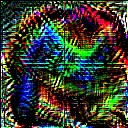
\includegraphics[width=0.2\textwidth]{Img/attack/x.jpg}} \qquad
%\subfigure{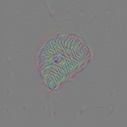
\includegraphics[width=0.2\textwidth]{Img/attack/z.jpg}}
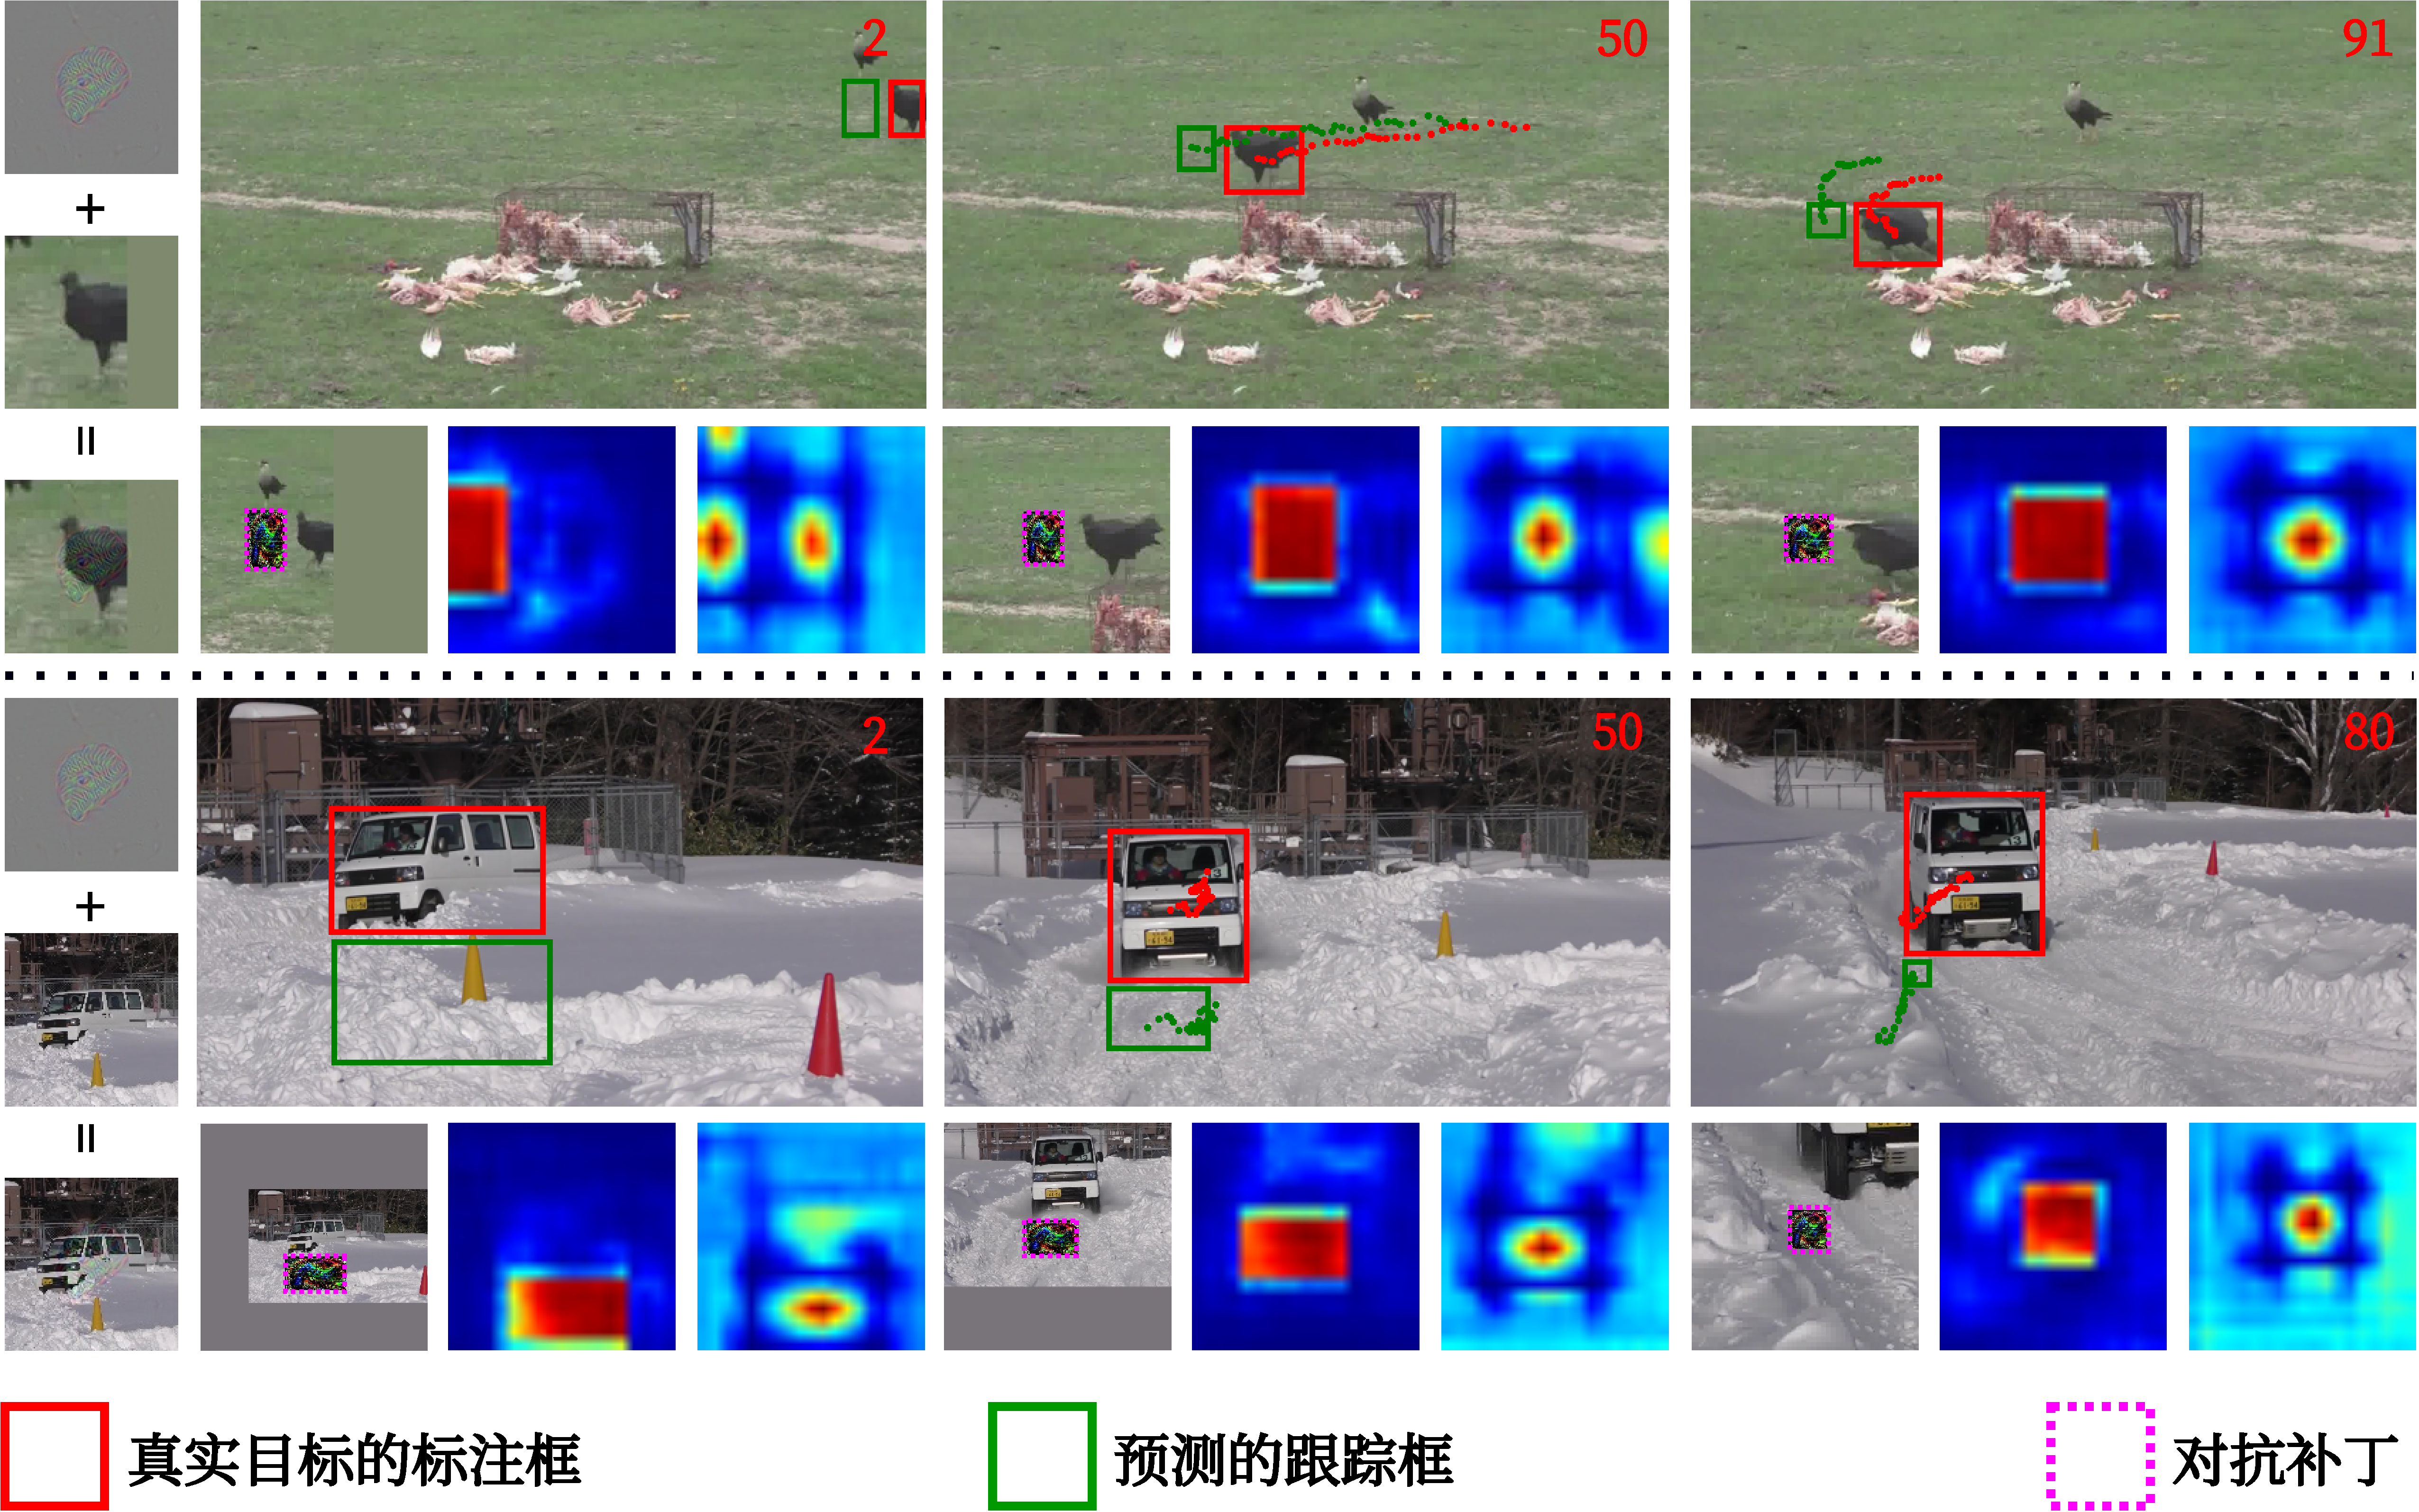
\includegraphics[width=1.0\textwidth]{Img/attack/1_v8.pdf}
\caption{An illustration of our attacks to SiamFC++ on some example tracking sequences from GOT-10k benchmark. Our approach generates the video-agnostic perturbations which can force SiamFC++ to follow a complicated trajectory at virtually no cost. This is realized by off-line training the perturbations so that the tracker mistakenly believes the \textit{fake target} area contains the object to be tracked (see the left heatmap). Moreover, the quality assessment branch in SiamFC++ is also misled to confirm this result (see the right heatmap). The \textit{fake target} size is gradually decreased.} 
%Being universal, the generated perturbations can be conveniently exploited to perturb videos on-the-fly without extra computations. 
%Red represents the ground-truth bounding box, and green represents the predicted bounding box by the tracker.
%The purple dashed box marks the universal adversarial patch. The left heatmap represents the probability of each spatial position to contain the \textit{fake target}, and the right heatmap represents the target state estimation quality.}
\label{fig:1}
\end{figure}

Recently, the robustness of Siamese trackers have attracted much attention in the sense of testing their vulnerability to adversarial attacks, and the focus has been directed towards more efficient and low-cost attacks \cite{TTP,FAN,SPARK}. Despite their success, these attack methods are not suitable for attacking the real-world online-tracking systems built upon the small edge platforms with limited computational resources. The reason is that they still need to craft the perturbations for each video independently based on either iterative optimisation or adversarial network inference, for which the adequacy of computational resources may be not ensured by the computationally intensive tracking systems. 

Universal adversarial perturbations (UAPs) proposed in \cite{UAP} can fool most images from a data distribution in an image-agnostic manner. Being universal, UAPs can be conveniently exploited to perturb unseen data on-the-fly without extra computations. Therefore, UAPs are particularly useful when attacking real-time applications deployed on platforms with limited computational resources. However, no existing work has touched the topic of attacking the Siamese trackers using UAPs, because it is hard to apply existing UAPs to attack Siamese trackers directly. The main reason lies in the fact that, (a) most UAPs are designed for typical neural networks with one image as input while Siamese networks accept both the template and search images, and (b) the goal of existing UAP methods is to disturb unary or binary model outputs for single instance while we need to use universal perturbations to mislead Siamese trackers to follow a specified trajectory.

In this paper, we make the first attempt in finding the video-agnostic perturbations that fool a state-of-the-art Siamese tracker, \ie, SiamFC++ \cite{SiamFC++}, in a targeted attack manner, which comes at virtually no cost in the online-tracking phase. Specifically, we aim to attack the trackers by adding a universal imperceptible perturbation to the template image and pasting a \textit{fake target}, \ie, a small universal adversarial patch, into the search image adhering to the predefined trajectory (as shown in Figure \ref{fig:1}), so that the tracker outputs the location and size of the \textit{fake target} instead of the real target. Our generated video-agnostic perturbations allow perturbing a novel video to come at no additional cost except the mere addition and pasting operations -- and not require gradient optimization or network inference. Experiment results on OTB2015 \cite{OTB}, GOT-10k \cite{GOT-10k} and LaSOT \cite{LaSOT} benchmarks demonstrate the effectiveness and efficiency of our approach.

\section{Related Work}

\subsection{Siamese Visual Tracking}

Siamese visual tracking is a fundamental research direction in template matching-based tracking besides the correlation filter-based methods. Both of them are aimed to "causally" estimate the positions of a template cropped from the initial video frame in the subsequent frames. Siamese trackers formulate visual tracking as learning cross-correlation similarities between a target template and the candidates in search region in a convolution fashion. Tracking is then performed by locating the object in the search image region based on the highest visual similarity. This paradigm is formulated as a local one-shot detection task.

Recently, some Siamese trackers~\cite{SiamRPN,SiamRPN++,SiamFC++} have demonstrated a significant performance improvement in visual tracking. 
In particular, SiamRPN \cite{SiamRPN} consists of one Siamese subnetwork for feature extraction and another region proposal subnetwork including the classification and regression branches separately. Based on its success in the decomposition of classification and state estimation, SiamRPN++ \cite{SiamRPN++} further breaks the restriction of strict translation invariance through a simple yet effective spatial aware sampling strategy and successfully trains a ResNet-driven Siamese tracker with significant performance gains. Apart from these anchor-based methods, an anchor-free tracker SiamFC++ \cite{SiamFC++} is further designed by considering non-ambiguous scoring, prior target scale/ratio distribution knowledge-free and estimation quality assessment guidelines.
In our experiments, we are focused on the anchor-free SiamFC++ tracker, whereas the transferability of our generated adversarial attacks to the previous anchor-based trackers is also studied.

\subsection{Adversarial Attacks}

Adversarial attacks to image classification were first investigated in \cite{intriguing}, which is aimed to identify the vulnerability of modern deep networks to imperceptible perturbations. 
%Recent studies also emerge to investigate the adversarial attacks to other diverse types of tasks such as natural language processing \cite{generating} and object detection \cite{wei2019transferable}.
Scenarios of possible adversarial attacks can be categorized along different dimensions.

\textit{Imperceptible Perturbations v.s. Adversarial Patch} The imperceptible perturbations most commonly modify each pixel by a small amount and can be found using a number of optimisation strategies such as Limited-memory BFGS \cite{intriguing} and PGD \cite{PGD}.
Different from the imperceptible perturbations, the adversarial patch is extremely salient to a neural network. The adversarial patch can be placed anywhere into the input image to cause the network to misbehave, and thus is commonly used for universal attacks \cite{patch}.
To the best of our knowledge, we are the first to attack object trackers utilizing both the imperceptible perturbation and the adversarial patch together, which are jointly trained in an end-to-end manner.
Note that our adversarial patch works in the network domain instead of the image domain. In the network-domain case, the noise is allowed to take any value and is not restricted to the dynamic range of image value as in the image-domain case \cite{karmon2018lavan}.

\textit{Untargeted Attacks v.s. Targeted Attacks} In the case of untargeted attacks, the adversary's goal is to cause the network to predict any incorrect label and whatever the incorrect label is does not matter, \eg, pushing the object location estimation just outside the true search region in visual tracking.
Targeted attacks, however, aim to change the network's prediction to some specific target label. In visual tracking, the targeted attacks aim to intentionally drive trackers to output specified object locations following a predefined trajectory.

\subsection{Adversarial Attacks in Visual Tracking}

Recently, there are several explorations of the adversarial attacks to the visual tracking task. For example, PAT \cite{PAT} generates physical adversarial textures via white-box attacks to steer the tracker to lock on the texture when a tracked object moves in front of it. However, PAT validates its method by attacking a light deep regression tracker GOTURN \cite{GOTURN}, which has low tracking accuracy on modern benchmarks. In this paper, we aim to attack the state-of-the-art Siamese trackers.
RTAA \cite{RTAA} takes temporal motion into consideration when generating lightweight perturbations over the estimated tracking results frame-by-frame. However, RTAA only performs the untargeted attacks for trackers, which is less challenging than the targeted attacks in this paper, as we aim to create arbitrary, complex trajectories at test time. 

Targeted attacks to follow an erroneous path which looks realistic are crucial to deceive the tracking system without raising any suspicion in the real-world applications.
SPARK \cite{SPARK} computes incremental perturbations by using information from the past frames to perform targeted attacks to Siamese trackers. However, SPARK needs to generate distinct adversarial example for every search image through heavy iterative schemes, which is time-consuming to attack online-tracking in real time. The recent real-time attacker in \cite{TTP} exclusively uses the template image to generate temporally-transferable perturbation in a one-shot manner, and then adds it to every search image. However, this method still needs to generate perturbations for each individual video, and its targeted attack setting requires diverse perturbations from several runs of network inference. It is ill-suited to attack a real-world online-tracking system when we can not get access to the limited computational resources. In this paper, however, we propose video-agnostic perturbations which allow perturbing a novel video to come at no additional cost except the mere addition and pasting operations.

\begin{figure}[t]
\centering
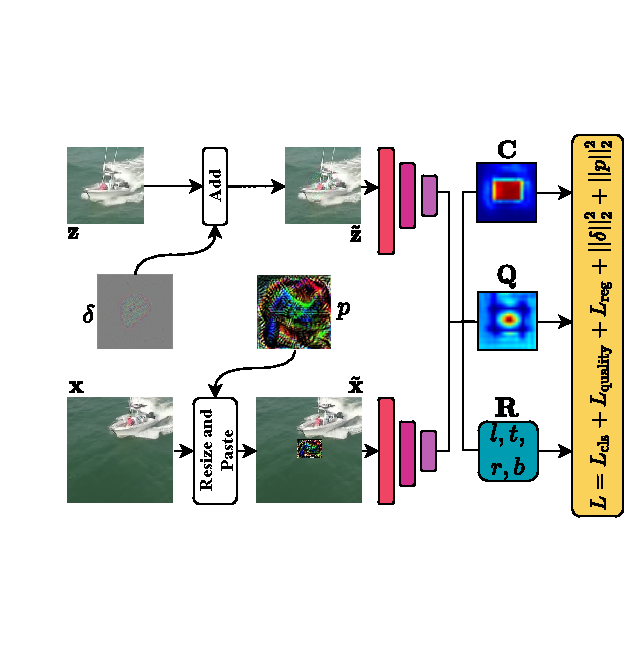
\includegraphics[width=1.0\textwidth]{Img/attack/network_v5.pdf}
\caption{The training pipeline of the proposed method. We aim to train an imperceptible perturbation $\delta$ for the template image $\textbf z$, and an adversarial patch $p$ for the search image $\textbf x$. After adding $\delta$ to $\textbf z$ and pasting the \textit{fake target} $p$ into $\textbf x$, the tracker outputs the location and size of the \textit{fake target} instead of the real target.}
\label{fig:net}
\end{figure}

\section{Method}

\textcolor{black}{In this section, we introduce our video-agnostic targeted attack framework for Siamese trackers. We aim to attack the tracker by adding an imperceptible perturbation to the template image and pasting a \textit{fake target}, i.e., an adversarial patch, into the search images adhering to the predefined trajectory, so that the tracker outputs the location and size of the \textit{fake target} instead of the real target. Below, we formalize our targeted attacks to SiamFC++ \cite{SiamFC++}, and then introduce our perturbation strategy in detail.}
 
\subsection{Problem Definition}

Let $V=\{I_i\}_1^T$ denote the frames of a video sequence of length $T$.
$B^{gt}=\{b^{gt}_i\}_1^T$ is used to represent the target's ground-truth position in each frame.
The visual object tracking aims to predict the position $B^{pred}=\{b^{pred}_i\}_1^T$ of this target in the subsequent frames given its initial state.
In SiamFC++, the tracker first transforms the paired reference frame $I_1$ and annotation $b_1^{gt}$ to get an template image $\textbf z$, and transforms the search frame $I_i$ to get the search image $\textbf x_i$ centered at the position estimated in the previous frame.
At each time-step, the template image $\textbf z$ and the search image $\textbf x_i$ are first passed individually through a shared backbone network, and the resulting features are processed by some non-shared layers and fused by depth-wise separable correlation. The fused features then act as input to a head network, which predicts a classification map $\textbf{C}$, a bounding box regression map $\textbf{R}$, and a quality assessment map $\textbf{Q}$ in an anchor-free manner. In short, $\textbf C$ encodes the probability of each spatial position to contain the target, $\textbf R$ regresses the bounding box of the target, and $\textbf Q$ predicts the target state estimation quality. The final bounding box is then generated according to $\textbf{C}$, $\textbf{R}$ and $\textbf{Q}$.

Formally, we aim to train an imperceptible perturbation $\delta$ for the template image $\textbf z$, and an adversarial patch $p$ for the search image $\textbf x_i$. After adding $\delta$ to $\textbf z$ and pasting the fake target $p$ into $\textbf x_i$, the tracker outputs the location and size of the adversarial patch instead of the real target (see Figure \ref{fig:net}).
Both $\delta$ and $p$ are universal (\ie, video-agnostic), which means perturbing a novel video only involves the mere addition and pasting of the perturbations to the template and search images -- and does not require gradient optimisation or network inference.

\subsection{Generating Video-Agnostic Perturbations}

In this subsection, we show how to train the video-agnostic perturbations $(\delta, p)$ for Siamese trackers.
During the $k$-th iteration of training, a video $V=\{I_i\}_1^T$ is randomly selected from the training dataset $\mathcal V$. Assuming the template perturbation at the $k$-th iteration is $\delta_k \in \mathbb{R}^{127\times 127 \times 3}$, and the adversarial patch is $p_k \in \mathbb{R}^{128\times 128\times 3}$. We first randomly pick paired frames $I_t, I_s$ from $V$.
The clean template image $\textbf z\in \mathbb{R}^{127\times 127 \times 3}$ is generated according to $I_t$ and $b^{gt}_t$, and the perturbed template image is:
\begin{equation}
\tilde {\textbf z} = \textbf z + \delta_k.
\end{equation}
Similarly, the clean search image $\textbf x \in \mathbb{R}^{303\times 303 \times 3}$ is generated according to $I_s$ and $b^{gt}_s$.
As mentioned before, the patch is regarded as a \textit{fake target} and pasted into the search images. We force the center position of the \textit{fake target} to near the center position of the real target within a shift range of 64 pixels, where shift is defined as the maximum range of translation generated from a uniform distribution.
The width/height of the \textit{fake target} is randomly selected between 32 pixels and 128 pixels.
The perturbed search image is generated as follows:
\begin{equation}
\tilde{\textbf x} = A(\textbf x, p_k, (l^x, l^y), (w, h)),
\end{equation}
where $(l^x, l^y)$ and $(w, h)$ represent the position and size of the \textit{fake target} with respect to the search image, respectively. $A$ is a patch application operator \cite{patch} which first resizes the patch $p_k \in \mathbb{R}^{128\times 128\times 3}$ to $\hat{p}_k \in \mathbb{R}^{w\times h\times 3}$, and then pastes the resized patch $\hat{p}_k$ into the search image $\textbf x$ at location $(l^x,l^y)$.

Subsequently, the SiamFC++ tracker $\phi(\cdot)$ takes $\tilde {\textbf x}$ and $\tilde{\textbf  z}$ as input and makes predictions as follows:
\begin{equation}
\textbf{C, R, Q} = \phi(\tilde {\textbf x}, \tilde{\textbf z}).
\end{equation}

\textit{Training Objective} The loss function is calculated as follows:
\begin{equation}
\begin{array}{l}
\begin{aligned}
L&=\frac{\alpha}{N_{\mathrm{pos}}} \sum_{x, y} L_{\mathrm{cls}}\left(\textbf{C}_{x, y}, \textbf{C}_{x, y}^{*}\right) \\
&+\frac{\beta}{N_{\mathrm{pos}}} \sum_{x, y} \textbf{1}_{\left\{\textbf{C}_{x, y}^{*}>0\right\}} L_{\mathrm{quality}}\left(\textbf{Q}_{x, y}, \textbf{Q}_{x, y}^{*}\right) \\
&+\frac{\gamma}{N_{\mathrm{pos}}} \sum_{x, y} \textbf{1}_{\left\{\textbf{C}_{x, y}^{*}>0\right\}} L_{\mathrm{reg}}\left(\textbf{R}_{x, y}, \textbf{R}_{x, y}^{*}\right) \\
&+\eta \cdot ||\delta_k||_2^2 +  \sigma \cdot ||p_k||^2_2,
\end{aligned}
\end{array}
\label{eq:loss}
\end{equation}
\textcolor{black} %(SiamFC++)
{where $\textbf{C}_{x, y}, \textbf{R}_{x, y}, \textbf{Q}_{x, y}$ represent the values of $\textbf{C}, \textbf{R}, \textbf{Q}$ at location $(x, y)$, respectively. $\textbf{C}^*, \textbf{R}^*, \textbf{Q}^*$ are the fake labels generated according to the position and size of the \textit{fake target}. $\textbf 1$ is the indicator function that takes 1 if the condition in subscribe holds and takes 0 if not, $N_{\mathrm{pos}}$ denotes the number of positive samples in the training phase, $L_{\mathrm{cls}}$ denotes the focal loss \cite{focal} for classification result, $L_{\mathrm{quality}}$ denotes the binary cross entropy (BCE) loss for quality assessment, and $L_{\mathrm{reg}}$ denotes the IoU loss \cite{iou-loss} for bounding box regression. Following SiamFC++, we assign 1 to $\textbf{C}_{x, y}^{*}$ if $(x, y)$ is considered as a positive sample, and 0 if as a negative sample.}

\iffalse
\begin{algorithm}[tb]
\caption{Training Process}
\label{alg:algorithm}
\textbf{Input}: Training dataset $\mathcal{V}$, Siamese tracker $\phi$, and max iteration number $N$.\\
\textbf{Output}: Imperceptible perturbation $\delta$, and adversarial patch $p$.
\begin{algorithmic}[1] %[1] enables line numbers
\STATE Let $k = 0$.
\WHILE{$k < N$}
\STATE Randomly pick a video $V\in \mathcal{V}$. The corresponding ground truth is $B^{gt}=\{b^{gt}_i\}^T_1$.
\STATE Randomly pick paired frames $I_t, I_s$ from $V$.
\STATE Generate template image $\textbf{z}$ according to $I_t$ and $b^{gt}_t$.
\STATE $\tilde{\textbf{z}} = \textbf{z} + \delta_k.$
\STATE Generate search image $\textbf{x}$ according to $I_s$ and $b^{gt}_s$.
\STATE Calculate the \textit{fake target} position $\{l^x, l^y, w, h\}$ with respect to the search image.
\STATE $\tilde{\textbf x} = A(\textbf x, p_k, (l^x, l^y), (w, h)).$
\STATE $\textbf{C, R, Q} = \phi(\tilde {\textbf x}, \tilde{\textbf z}).$
\STATE Generate fake labels $\textbf{C}^*,\textbf{R}^*,\textbf{Q}^*$ using $\{l^x, l^y, w, h\}$.
\STATE Calculate loss $L(\textbf{C, R, Q}, \textbf{C}^*, \textbf{R}^*, \textbf{Q}^*)$ using Equ. \ref{eq:loss}.
\STATE $\delta_{k+1} = \delta_{k} - \epsilon_1 \cdot \text{sign}(\nabla_{\delta_k}L).$
\STATE $p_{k+1} = p_{k} - \epsilon_2 \cdot \text{sign}(\nabla_{p_k}L).$
\STATE $k = k + 1.$
\ENDWHILE
\STATE \textbf{return} $\delta_N, p_N.$
\end{algorithmic}
\label{alg}
\end{algorithm}
\fi

\begin{figure*}[t]
\centering
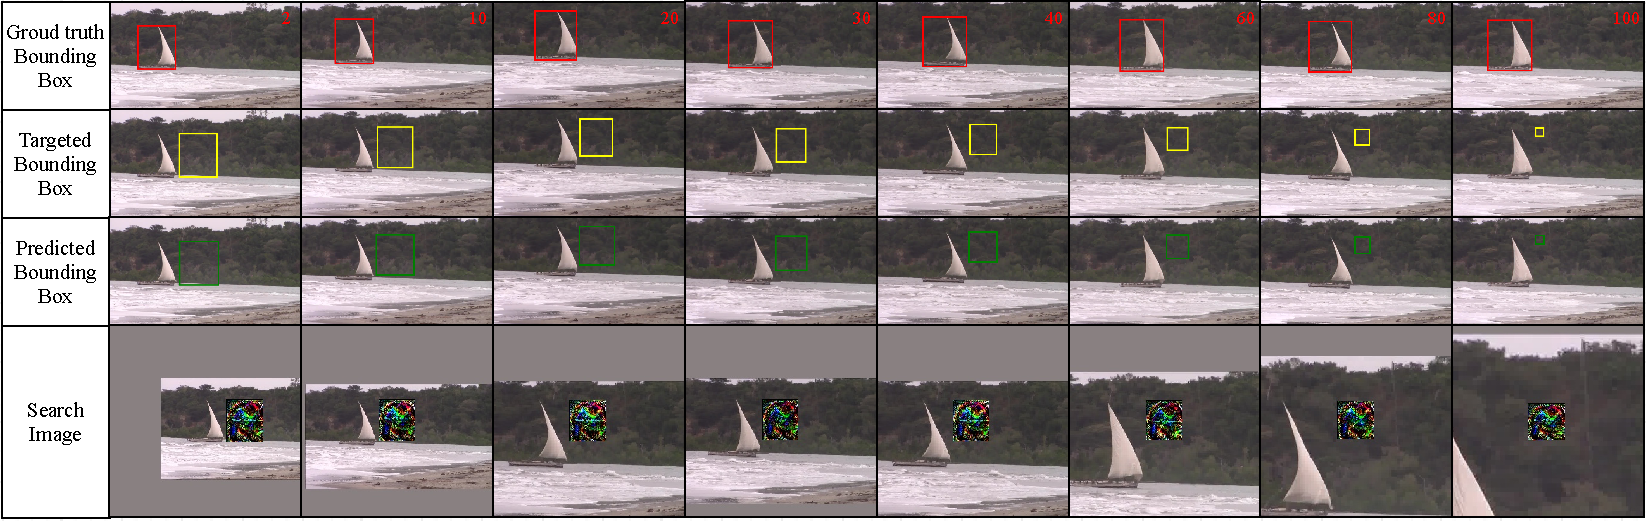
\includegraphics[width=1.0\textwidth]{Img/attack/vis_v4.pdf}
\caption{Our targeted attack results following a predefined \textit{fake trajectory} (indicated by the yellow targeted bounding box).}
\label{fig:vis}
\end{figure*}

\textit{Optimisation} At each training step, the perturbations are updated as follows:
\begin{gather}
\delta_{k+1} = \delta_{k} - \epsilon_1 \cdot \text{sign}(\nabla_{\delta_k}L)\\
p_{k+1} = p_{k} - \epsilon_2 \cdot \text{sign}(\nabla_{p_k}L),
\end{gather}
where $\epsilon_1$ is used to ensure that the perturbation added to the template image is imperceptible, and $\epsilon_2$ is used to maintain the training stability.
During training, we only optimize the values of perturbations $(\delta, p)$ and the parameters of the Siamese network remain intact.

We outline this training procedure in Algorithm \ref{alg}.

\subsection{Attacking the Tracker at Inference Time}

Once the perturbations $(\delta, p)$ is trained, we can use them to perturb the template image and search images of any novel video for attacking. Both $\delta$ and $p$ are universal (i.e., video-agnostic), which means perturbing a novel video only involves the mere addition and pasting of the perturbations to the template and search images -- and does not require gradient optimisation or network inference.
Assume $B^{fake}=\{b^{fake}_i\}_1^{T}$ is the trajectory we hope the tracker to output.
During tracking the $i$-th frame of the video $V=\{I_i\}_1^T$, we need to transform the bounding box $b^{fake}_i$ (with respect to the original frame $I_i$) into the box $\hat b_i=\{l^x_i, l^y_i, w_i, h_i\}$ with respect to the search image $\textbf x_i$, and paste $p$ into $\textbf x_i$ according to $\hat b_i$:
\begin{equation}
\tilde{\textbf x}_i = A(\textbf x_i, p, (l^x_i, l^y_i), (w_i, h_i)).
\end{equation}
The tracker then takes $\tilde{\textbf z}_i=\textbf z_i+\delta$ and $\tilde{ \textbf x}_i$ as input, and the subsequent tracking procedure remains the same as SiamFC++.

%%%%%%%%%%%%%%%%%%%%%%%%%%%%%%%
%%%%%%%%%%%%%%%%%%%%%%%%%%%%%%%
\section{Experiments}

\subsection{Experimental Setup}

\textit{Evaluation Benchmarks} We evaluate our video-agnostic perturbations for targeted attacks on several tracking benchmarks, \ie, OTB2015 \cite{OTB}, GOT-10k \cite{GOT-10k}, and LaSOT \cite{LaSOT}. Generally speaking, OTB2015 is a typical tracking benchmark which is widely used for evaluation for several years, GOT-10k has the advantage of magnitudes wider coverage of object classes, and LaSOT has much longer video sequences with average duration of 84 seconds. They all follow the One-Pass Evaluation (OPE) protocol and their evaluation methodologies are similar as the measurement is mostly based on the success and precision of the trackers over the test videos. For instance, they all measure the success based on the fraction of frames in a sequence where the intersection-over-union (IoU) overlap of the predicted and ground truth rectangles exceeds a given threshold, and then the trackers are ranked using the area-under-the-curve (AUC) criterion. Since the average of IoU overlaps (AO) over all the test video frames is recently proved to be equivalent to the AUC criterion, we thus denote the success measurement as AO in the following. Besides AO, a success rate (SR) metric is also directly used to measure the percentage of successfully tracked frames given a threshold as in GOT-10k. As for the precision, it encodes the proportion of frames for which the center of the predicted rectangle is within 20 pixels of the ground truth center. Since the precision metric is sensitive to the resolution of the images and the size of the bounding boxes, a metric of normalized precision over the size of the ground truth bounding box is proposed and the trackers are then ranked using the AUC for normalized precision between 0 and 0.5.

\textit{Generating the Fake Trajectory} We need to predefine a specific trajectory $B^{fake}=\{b^{fake}_i\}_1^{T}$ for each video to achieve targeted attack in the online-tracking phase, which we call the \textit{fake trajectory}. We denote the \textit{real trajectory} as $B^{gt}=\{b^{gt}_i\}_1^T$ with the bounding box ground truth.
It is possible to manually label arbitrary $B^{fake}$ for each video, however, it will be time-consuming in our experimental evaluation. So we generate $B^{fake}$ based on $B^{gt}$. Specifically, the \textit{fake trajectory} follows the \textit{real trajectory} and the adjacent boundaries of $b^{fake}_i$ and $b^{gt}_i$ are 16 pixels apart.
%The size of $b^{fake}_0$ is the same as $B^{gt}_0$ and the size of $b^{fake}_i$
The bounding box size of the \textit{fake trajectory} gradually changes from the size of $b^{gt}_1$ to $64\times 64$. Note that the annotations of GOT-10k's test data are kept private, so we only use its validation set for our evaluation and denote it as GOT-Val.

\textit{Image Quality Assessment} We use structural similarity (SSIM) \cite{SSIM} to evaluate the quality of the generated imperceptible template perturbation $\delta$. It is difficult to be found when SSIM is close to 1 (see Table \ref{tab:iter}).

\begin{table}
\centering
%\scriptsize
\footnotesize
\tabcolsep=2.0pt
%\resizebox{0.48\textwidth}{!}{%
\begin{tabular}{c c | c | c | c}
\toprule
\multirow{2}{*}[-2pt]{Benchmarks} & \multirow{2}{*}[-2pt]{Metrics} & Clean Videos    & \multicolumn{2}{c}{Perturbed Videos}  \\
\cmidrule{3-5}
                          &                         & Real Traj. & Real Traj. & Fake Traj.     \\ 
\midrule
\multirow{2}{*}{OTB-15} 
& AO   & 0.642 & 0.035 & 0.842\\
& Precision & 0.861 & 0.048 & 0.928\\
\midrule
\multirow{2}{*}{GOT-Val} 
& SR & 0.897 & 0.023 & 0.890\\
& AO 				   & 0.760 & 0.035 & 0.818 \\
\midrule
\multirow{3}{*}{LaSOT} 
& Precision       & 0.514 & 0.013 & 0.820\\
& Norm. Prec. & 0.551 & 0.015 & 0.788\\
& AO & 0.525 & 0.022 & 0.767\\
%& Succ. rate  & 0.626 & 0.016 & 0.834\\
\midrule
\multicolumn{2}{c|}{FPS} & 58 & 58 & 58\\
\bottomrule
\end{tabular}
%}
\caption{Overall attack results on the evaluation benchmarks.}
\label{tab:benchmark results}
\end{table}

\subsection{Implementation Details}

In our evaluation, the backbone Siamese network of our base tracker SiamFC++ \cite{SiamFC++} adopts GoogLeNet \cite{GoogLeNet}.
We implement our approach in Pytorch and train our perturbations using three GTX 1080Ti GPUs.
We adopt COCO \cite{COCO}, ILSVRC-VID \cite{VID} and the training splits of GOT-10k \cite{GOT-10k} and LaSOT \cite{LaSOT} as our training set.
We train the perturbations for 32768 iterations with a mini-batch of 96 images (32 images per GPU).
The learning rate of the template perturbation $\epsilon_1$ is set to 0.1, and for the adversarial patch it is $\epsilon_2 = 0.5$.
We generate training samples following the practice in SiamFC++.
During both the training and online-tracking phase, the off-the-shelf SiamFC++ tracking network model\footnote{It is exclusively trained on the training split of GOT-10k by the authors of SiamFC++ and can be downloaded from \url{https://drive.google.com/file/d/1BevcIEZr_kgyFjhxayOFw08DFl2u5Zi7/view}} is fixed and used for the whole evaluation, the spatial size of the template image is set to $127\times 127$, and the search image is $303\times 303$.
In Equ. \ref{eq:loss}, we set $\alpha=1, \beta=1, \gamma=1, \eta=0.005$, and $\sigma=10^{-5}$.

\begin{table}
\centering
%\scriptsize
\footnotesize
\tabcolsep=2.5pt
%\resizebox{0.48\textwidth}{!}{%
\begin{tabular}{ccc|cc|cc} 
\toprule
\multirow{2}{*}[-2pt]{$L_{\text{cls}}$}     & \multirow{2}{*}[-2pt]{$L_{\text{quality}}$} & \multirow{2}{*}[-2pt]{$L_{\text{reg}}$} & \multicolumn{2}{c|}{Fake Traj.}          & \multicolumn{2}{c}{Real Traj.}           \\ 
\cmidrule{4-7}
                       &                    &                    & AO                    & SR                    & AO                    & SR                     \\ 
\midrule
\checkmark   &    &    & 0.718  & 0.824    & 0.086 & 0.083   \\
   & \checkmark   &    & 0.044  & 0.044    & 0.703 & 0.842   \\
   &    & \checkmark   & 0.664  & 0.726    & 0.165 & 0.184   \\
\checkmark   & \checkmark   & \checkmark   & 0.818  & 0.890    & 0.035 & 0.023   \\ \bottomrule
\end{tabular}
%}
\caption{Contribution of each loss on GOT-Val.}
\label{tab:loss}
\end{table}

\subsection{Attack Results on the Evaluation Benchmarks}

\textit{Overall Attack Results} We test the performance of our targeted attack method on the evaluation benchmarks and gather the overall results in Table \ref{tab:benchmark results}. It is shown that the base tracker SiamFC++ can achieve state-of-the-art performance on all the evaluation benchmarks and run in real time (at about 58 fps on an GTX 1080Ti GPU). However this real-time performance requires the computationally intensive tracking system to occupy most of the computational resources, and thus it is appealing to develop a virtually costless attack method to fool the tracking system without scrambling for the resources. As shown in Table \ref{tab:benchmark results}, our attack method can satisfy this appealing demand and fool the SiamFC++ tracker effectively by misleading the tracker to follow a predefined \textit{fake trajectory}. Moreover, the high AO and Precision performance with respect to the \textit{fake trajectory} indicates a more effective attack without raising any suspicion (see Figure \ref{fig:vis}).

\begin{table*}
\centering
%\scriptsize
\footnotesize
\tabcolsep=3.0pt
%\resizebox{\textwidth}{!}{%
\begin{tabular}{cc|cccccccccccccccc} 
\toprule
\multicolumn{2}{c|}{Iterations}     & 1     & 2     & 4     & 8     & 16    & 32    & 64    & 128   & 256   & 512   & 1024  & 2048  & 4096  & 8192  & 16384 & 32768  \\ 
\midrule
\multirow{2}{*}{Fake Traj.} & AO    & 0.002 & 0.002 & 0.002 & 0.002 & 0.002 & 0.003 & 0.007 & 0.042 & 0.299 & 0.668 & 0.746 & 0.781 & 0.798 & 0.820 & 0.821 & 0.818  \\
                                 & SR    & 0.000 & 0.000 & 0.000 & 0.000 & 0.000 & 0.001 & 0.005 & 0.044 & 0.335 & 0.749 & 0.822 & 0.855 & 0.872 & 0.895 & 0.897 & 0.890  \\ 
\midrule
\multirow{2}{*}{Real Traj.} & AO    & 0.757 & 0.756 & 0.757 & 0.757 & 0.758 & 0.759 & 0.753 & 0.720 & 0.474 & 0.150 & 0.095 & 0.071 & 0.041 & 0.032 & 0.032 & 0.035  \\
                                 & SR    & 0.894 & 0.891 & 0.893 & 0.891 & 0.893 & 0.896 & 0.888 & 0.852 & 0.559 & 0.164 & 0.098 & 0.066 & 0.031 & 0.021 & 0.022 & 0.023  \\ 
\midrule
\multicolumn{2}{c|}{SSIM of $\delta$}                        & 1.00  & 1.00  & 1.00  & 1.00  & 0.99  & 0.99  & 0.97  & 0.93  & 0.86  & 0.86  & 0.87  & 0.88  & 0.88  & 0.88  & 0.88  & 0.88   \\
%\multicolumn{2}{c|}{MSE}                         & 0.51  & 0.26  & 0.32  & 0.37  & 0.48  & 0.84  & 2.03  & 5.65  & 15.10 & 25.43 & 23.70 & 21.89 & 20.69 & 20.49 & 20.03 & 20.87  \\
\bottomrule
\end{tabular}
%}
\caption{Influence of the training iteration number on GOT-Val.}
\label{tab:iter}
\end{table*}

\begin{table}
\centering
%\scriptsize
\footnotesize
\tabcolsep=2.0pt
%\resizebox{0.48\textwidth}{!}{%
\begin{tabular}{c|cc|cc|cc} 
\toprule
\multirow{3}{*}[-6pt]{Backbone} & \multicolumn{2}{c|}{Clean Videos}    & \multicolumn{4}{c}{Perturbed Videos}                                        \\ 
\cmidrule{2-7}
                          & \multicolumn{2}{c|}{Real Traj.} & \multicolumn{2}{c|}{Real Traj.} & \multicolumn{2}{c}{Fake Traj.}  \\ 
\cmidrule{2-7}
                          & AO    & SR                           & AO    & SR                           & AO    & SR                           \\ 
\midrule
GoogLeNet                 & 0.760 & 0.897                        & 0.035 & 0.023                        & 0.818 & 0.890                        \\
AlexNet                   & 0.720 & 0.850                        & 0.196 & 0.227                        & 0.572 & 0.640                        \\
ShuffleNet                & 0.766 & 0.888                        & 0.554 & 0.656                        & 0.135 & 0.134                        \\
\bottomrule
\end{tabular}
%}
\caption{Transferability to different backbones on GOT-Val.}
\label{tab:backbone}
\end{table}

\begin{table}
\centering
%\scriptsize
\footnotesize
\tabcolsep=2.0pt
%\resizebox{0.48\textwidth}{!}
\caption{Transferability to different tracking architectures on OTB2015.}
\label{tab:arch}
\end{table}

\textit{Ablation Study: Influence of Training Loss} We implement a series of experiments to analyse and evaluate the contribution of each loss component.
In Table \ref{tab:loss}, we report our results on GOT-Val with respect to different perturbations trained with different combinations of loss terms in Equ. \ref{eq:loss}.
To summarize, all the loss terms are beneficial whereas the classification term is more important than the quality assessment term for attacking.

\textit{Ablation Study: Influence of Training Iterations} As shown in Table \ref{tab:iter}, after around 30000 training iterations, the generated perturbations can fool most targets in GOT-Val. The AO with respect to the \textit{real trajectory} falls down from 0.760 to 0.035. We notice that at the start of training period (when training iteration number is less than 2048), the decreasing of AO is significantly faster than in the later period. This demonstrates the fast convergence ability of our end-to-end training pipeline while generating the adversarial perturbations.

\subsection{Transferability Analysis}

\textit{Transferability to Different Backbones} We evaluate the transferability of our attacks when applying the perturbations to two more different backbones of SiamFC++, \ie, ShuffleNet \cite{ShuffleNet} and AlexNet \cite{AlexNet}.
The experimental results are shown in Table \ref{tab:backbone}. In the case of SiamFC++-AlexNet, the AO with respect to the \textit{real trajectory} drops from 0.72 to 0.196. However, our perturbations do not generalize well to SiamFC++-ShuffleNet, which we conjecture to be due to the particular group convolution and channel shuffle operations in ShuffleNet.

\textit{Transferability to Different Tracking Architectures} We evaluate the transferability of our attacks when applying the perturbations to two more state-of-the-art anchor-based trackers: AlexNet-based SiamRPN \cite{SiamRPN} and ResNet-based SiamRPN++ \cite{SiamRPN++} to verify the transferability to different tracking architectures.
SiamRPN uses an RPN network to perform location regression and target classification on the response maps. SiamRPN++ performs layer-wise and depth-wise aggregation to improve accuracy based on the effective training using the ResNet backbone. The experimental results are shown in Table \ref{tab:arch}. In the case of SiamRPN, the AO with respect to the \textit{real trajectory} drops from 0.666 to 0.379 while the performance of SiamRPN++ is decreased from 0.676 to 0.518. The results show good transferability of our attacks to different tracking architectures, even if the generated perturbations are applied to anchor-based trackers.

\subsection{Comparison with Other Methods}

We compare the attack performance of our method with the recent promising attack approaches, \ie, the untargeted attack method CSA \cite{CSA} based on AlexNet and two other targeted attack methods FAN \cite{FAN} based on AlexNet and TTP \cite{TTP} based on ResNet-50.
We report the precision score with respect to the \textit{real / fake trajectory} in Table \ref{tab:untargeted}.
Our method significantly outperforms other methods at no additional cost except the mere addition and pasting operations -- and does not require gradient optimization or network inference.

\begin{table}[]
\centering
\footnotesize
\tabcolsep=2.0pt
\begin{tabular}{@{}cccccc@{}}
\toprule
\multirow{2}{*}[-2pt]{Method} & \multirow{2}{*}[-2pt]{Tracker} & \multirow{2}{*}[-2pt]{\begin{tabular}[c]{@{}c@{}}Attack\\ Cost(ms)\end{tabular}} & \multirow{2}{*}[-2pt]{\begin{tabular}[c]{@{}c@{}}Clean\\ Videos\end{tabular}} & \multicolumn{2}{c}{Perturbed Videos} \\ \cmidrule(l){5-6} 
 &  &  &  & Real Traj. & Fake Traj. \\ \midrule
CSA & SiamRPN & 4720 & 0.851 & 0.458 & - \\
FAN & SiamFC & 10 & 0.720 & 0.180&0.420 \\
TTP & SiamRPN++ & 8 & 0.910 & 0.080&0.692 \\
\midrule
Ours & SiamFC++ & 0 & 0.861 & 0.048&0.928 \\ \bottomrule
\end{tabular}%
\caption{Precision score with respect to the \textit{real / fake trajectory} on OTB2015.}
\label{tab:untargeted}
\end{table}

\section{Conclusion}

In this paper, we propose a video-agnostic targeted attack method for Siamese trackers. 
We aim to attack the tracker by adding an imperceptible perturbation to the template image and pasting a \textit{fake target}, \ie, a small adversarial patch, into the search image adhering to the predefined trajectory, so that the tracker outputs the location and size of the \textit{fake target} instead of the real target. Being universal, the generated perturbations can be conveniently exploited to perturb videos on-the-fly without extra computations.
Experiments on several popular datasets show that our method can effectively fool the Siamese trackers in a targeted attack manner.